\documentclass{beamer}
\usepackage{csquotes}
\usepackage{hyperref}
\usepackage{graphicx}
\graphicspath{ {./assets} }
% \setbeameroption{show notes}
% \setbeameroption{show only notes}

\title{Git and Github}
\author{Edwin Kofler}
% \institute{Edwin Kofler}
% \date{Fall 2022}
\hypersetup{
	colorlinks=true
}

\begin{document}
\frame{\titlepage}

\begin{frame}
	\begin{columns}
		\begin{column}{0.48\textwidth}
			
\includegraphics{panda-500px.jpg} \newline
			{ \tiny Image by Art G. on \href{https://www.flickr.com/photos/digitalart/4084550022}{Flickr}; licensed as CC BY-NC-ND 2.0 }
	  \end{column}
	  \begin{column}{0.48\textwidth}
			{\Huge Edwin Kofler} \newline
			\begin{itemize}
				\item \href{https://edwinkofler.com/}{Website}
				\item \href{https://github.com/hyperupcall}{GitHub}
				\item \href{https://twitter.com/hyperupcall}{Twitter}
				\item \href{https://www.linkedin.com/in/hyperupcall}{LinkedIn}
			\end{itemize}
	  \end{column}
	\end{columns}
\end{frame}

\begin{frame}{Agenda}
	\begin{enumerate}
		\item Introduce Git and Github
		\item Tour GitHub (create account, explore site)
		\item Download Git and GitHub Desktop
		\item Make a GitHub Contribution
		\item Bonus Points: Using Git over the Command Line
		\item Resources
	\end{enumerate}

	\note{
		This priority of this workshop is hands-on experience with GitHub.

		Learn by doing, rather than just watching someone talk or explain
	}
\end{frame}


\begin{frame}{Introducing Git}

	From the official Git \href{https://git-scm.com}{website}: \newline

	\begin{displayquote}
		Git is a \href{https://git-scm.com/about/free-and-open-source}{free and open source} distributed version control system...
	\end{displayquote}

	{
		\small

		But what does that mean in practice? Git...

		\begin{itemize}
			\item Lets you ``look at" a file at a previous point in time
			\item Allows multiple people to work on the same codebase at a time
			\item Lets you experiment with your code (and keep the original copy safe)
		\end{itemize}
	}
	
	\href{https://raw.githubusercontent.com/ecc-cs-club/slides/main/1-Git-And-GitHub/assets/using-git.png}{
		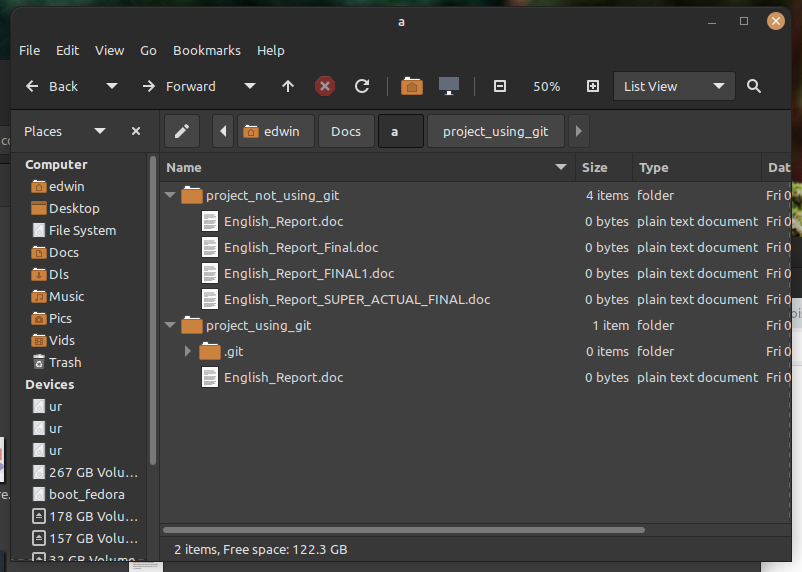
\includegraphics[width=6cm]{using-git.png}
	}
	

	\note{
		multiple people to work - if no git, would have to work on same computer. sometimes have trouble opening up files
		history - from a ``single file" to many many files like in those big projects
	}
\end{frame}


\begin{frame}{Introducing GitHub}
	\begin{itemize}
		\item Sort of a combination of Dropbox and Twitter
		\item Better to show, than tell...
	\end{itemize}

	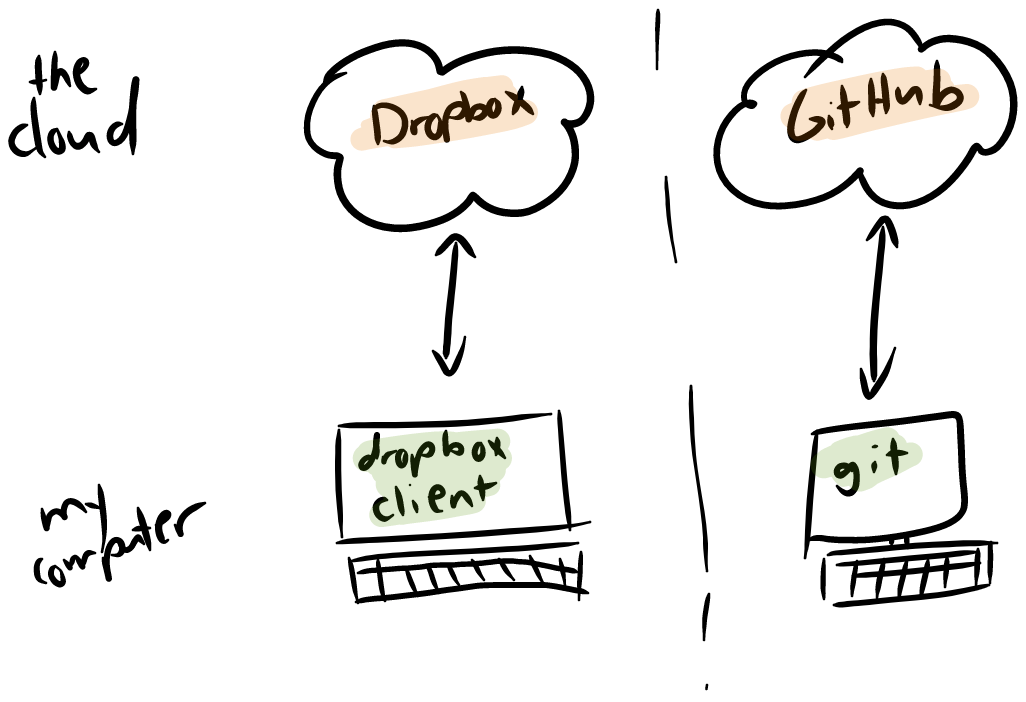
\includegraphics[width=10cm]{dropbox-github.png} \newline

	\note{
		Like Dropbox, sort of ``syncing" a folder on your computer with a remote server

		There is a \href{https://docs.github.com/en/get-started/signing-up-for-github/signing-up-for-a-new-github-account}{help page}, but it does not offer useful information
	}
\end{frame}

\begin{frame}{Tour of GitHub}
	\begin{itemize}
		\item Create GitHub account
		\item Explore ``home" view
		\item Show ``profile" view
		\item Create a ``profile README"
		\item Show small repository: \href{https://github.com/hyperupcall/website}{hyperupcall/website}
		\item Show large repository: \href{https://github.com/xournalpp/xournalpp}{xournalpp/xournalpp}
	\end{itemize}

	\note{
		- in issues: ``good first issue"
		- show pull requests
	}
\end{frame}


\begin{frame}
	\frametitle{Downloading Git and GitHub}

	Git must be installed before using GitHub Desktop
	\newline

	\begin{itemize}
		\item For \textbf{Git}
			\begin{itemize}
				\item Go to \href{https://git-scm.com/}{git-scm.com}
				\item See middle-right part of page for download button
			\end{itemize}
		\item For \textbf{GitHub Desktop}
			\begin{itemize}
				\item Go to \href{https://desktop.github.com}{desktop.github.com} (Linux users, see \href{https://github.com/shiftkey/desktop/releases}{shiftkey/desktop})
				\item See download button
			\end{itemize}
	\end{itemize}
\end{frame}

\begin{frame}{Make a GitHub Contribution}
	\begin{enumerate}
		\item Find a repository to contribute too (ex. \href{https://github.com/ecc-cs-club/practice}{ecc-cs-club/practice})
		\item Find an issue to ``fix" (optional)
		\item Fork the repository (usually required)
		\item Clone your ``forked" repository to your computer with a Git client (ex. GitHub Desktop)
		\item Open the repository with a code editor (ex. VSCode)
		\item Make the code or text changes required
		\item Make a Git commit, then push your changes
		\item Create a Pull Request (PR)
		\item Wait
	\end{enumerate}
\end{frame}

\begin{frame}
	\frametitle{Resources}

	\begin{itemize}
		\item \href{https://www.youtube.com/watch?v=BCQHnlnPusY&list=PLRqwX-V7Uu6ZF9C0YMKuns9sLDzK6zoiV}{The Coding Train: Git}
		\item \href{https://www.youtube.com/watch?v=USjZcfj8yxE}{Using Git on the command line (video)}
		\item \href{https://education.github.com/git-cheat-sheet-education.pdf}{Git cheatsheet by GitHub}
		\item \href{https://about.gitlab.com/images/press/git-cheat-sheet.pdf}{Git cheatsheet by GitLab}
		\item \href{https://www.youtube.com/watch?v=yr6IzOGoMsQ}{Video: How to contribute to GitHub}
	\end{itemize}
\end{frame}
\end{document}
